\definecolor{color1}{RGB}{145,30,180}
\definecolor{color2}{RGB}{245,130,48}
\definecolor{color3}{RGB}{230,25,75}

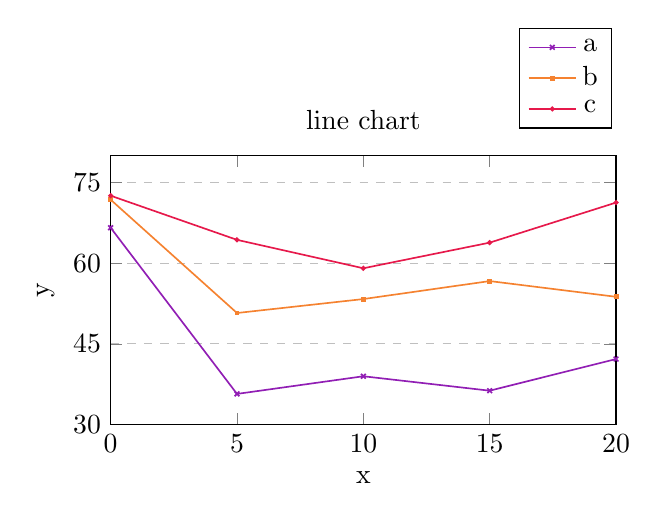
\begin{tikzpicture} %tikz图片
\scalefont{0.7} %设置字体大小
\begin{axis}[
sharp plot, %控制线的风格
title=line chart,%图像标题
xmode=normal,% 控制坐标轴为线性
%		ymode=log,% 控制坐标轴为对数
xlabel=x, %x坐标名
ylabel=y, %y坐标名
width=8cm, height=5cm,  %设置长和宽
xmin=0,xmax=20,  % 设置x坐标范围
ymin=30, ymax=80,  % 设置y坐标范围
xtick={0,5,10,15,20}, %指定x轴刻度值。如果为空,则自动设置刻度线。即分割坐标轴
ytick={30,45,60,75}, %指定y轴刻度值。如果为空,则自动设置刻度线。即分割坐标轴
xlabel near ticks, % 设置x坐标名位置靠近折线图
ylabel near ticks, % 设置y坐标名位置靠近折线图
ymajorgrids=true, % 启用/禁用 [公式] 轴上刻度线位置上的网格线
grid style=dashed, % 设置网格线格式
legend style={at={(0.9,1.1)},anchor=south}, % 设置标签位置
%			legend columns=3, %设置标签列数
%			legend pos=north west, % 设置折线对应标签的位置
%			legend style={nodes={scale=0.6, transform shape}},  % 设置折线标签的格式
]

%画第一条线,semithick设置线的粗细为0.6pt,mark是折线标示形状,options是mark形状的大小 , olive!50!white是颜色,coordinates中包含要绘制的点的坐标
\addplot+[semithick,mark=x,mark options={scale=0.6}, color=color1] plot coordinates { 
    (0,66.58)
    (5,35.71)
    (10,38.99)
    (15,36.31)
    (20,42.19)
};
\addlegendentry{a}%第一条线标签

%画第二条线
\addplot+[semithick,mark options={scale=0.3}, color=color2] plot coordinates {
    (0,71.79)
    (5,50.74)
    (10,53.33)
    (15,56.67)
    (20,53.75)
};
\addlegendentry{b} %第二条线标签

%画第三条线
\addplot+[semithick,mark options={scale=0.3}, color=color3] plot coordinates {
    (0,72.53)
    (5,64.33)
    (10,59.05)
    (15,63.81)
    (20,71.25)
};
\addlegendentry{c} %第三条线标签

\end{axis}
\end{tikzpicture}